\section[Исследование распределения Максвелла]{Исследование распределения Максвелла}

\textit{\textbf{Начальные параметры:}}
\begin{center}
    \begin{tabular}{c}
    \begin{lstlisting}
(* Constants *)
k = 1.380649 * 10^-23; (*Boltzmann constant*)
H2m = 2 * 1.6605 * 10^-27; 
N2m = 28 * 1.6605 * 10^-27;
O2m =  32 * 1.6605 * 10^-27;
T0 = 73;
T1 = 273;
T2 = 473;
    \end{lstlisting}
    \end{tabular}
\end{center}

% Часть A

\textit{\textbf{(a) Исследование распределения Максвелла по модулю скорости}}  
\begin{equation*}
    f(v) = 4\pi v^{2} (\frac{m}{2\pi kT})^{3/2} exp(-\frac{mv^{2}}{2kT})
\end{equation*}


Листинг программы Matematica (\textbf{Plot} для $T_{0}$, для $T_{1}, T_{2}$ аналогично):
\begin{center}
    \begin{tabular}{c}
    \begin{lstlisting}
(* Maxwell Distribution for the absolute value of speed *)
FMaxwellDistAbs[m_, v_, T_] =
    4*Pi*v^2*(m/(2*Pi*k*T))^(3/2)*Exp[-m*v^2/(2*k*T)];

(* T = T0 = 73K *)
Plot[{FMaxwellDistAbs[H2m, v, T0], 
      FMaxwellDistAbs[N2m, v, T0],
      FMaxwellDistAbs[O2m, v, T0]},
     {v, 0, 5000},
     PlotLegends -> "Expressions",
     AxesLabel -> {v, f[v]},
     PlotRange -> All]
    \end{lstlisting}
    \end{tabular}
\end{center}

\newpage
Полученные графики распределения Максвелла по модулю скорости:
\hspace{0pt}
\begin{figure}[H]
    \begin{minipage}[h]{0.47\linewidth}
        \center{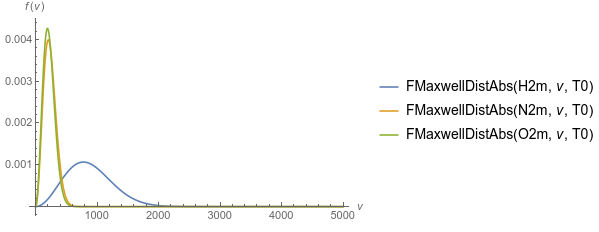
\includegraphics[width=1\linewidth]{1_1_maxw_abs_t0.png}}\\
        $T=T_{0}=73K$
    \end{minipage}
    \hfill
    \begin{minipage}[h]{0.47\linewidth}
        \center{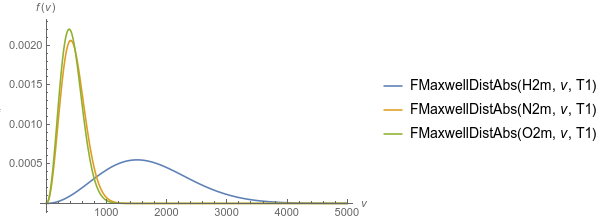
\includegraphics[width=1\linewidth]{1_2_maxw_abs_t1.png}}\\
        $T=T_{1}=273K$
    \end{minipage}
    \vfill
    \vspace{6pt}
    \centering 
    \begin{minipage}[h]{0.47\linewidth}
        \center{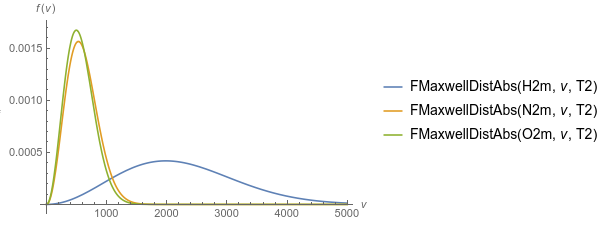
\includegraphics[width=1\linewidth]{1_3_maxw_abs_t2.png}}\\
        $T=T_{2}=473K$
    \end{minipage}
\end{figure}

% Часть B

\textit{\textbf{(b) Исследование распределения Максвелла по проекции скорости}}  
\begin{equation*}
    f(v_{i}) = \sqrt{\frac{m}{2\pi kT}}\space exp(-\frac{mv_{i}^{2}}{2kT})
\end{equation*}


Листинг программы Matematica (так как распределение аналогично для всех трех проекций, визуализируем для произвольной):
\begin{center}
    \begin{tabular}{c}
    \begin{lstlisting}
(* Maxwell Distribution for the speed component in 3-dim space *)
FMaxwellDistSpComp[m_, vi_, T_] =
   Sqrt[m/(2*Pi*k*T)]*Exp[-m*vi^2/(2*k*T)];

Plot[{FMaxwellDistSpComp[H2m, v, T0],
      FMaxwellDistSpComp[N2m, v, T0],
      FMaxwellDistSpComp[O2m, v, T0]},
     {v, -5000, 5000},
     PlotLegends -> "Expressions",
     AxesLabel -> {v, f[v]},
     PlotRange -> All]
    \end{lstlisting}
    \end{tabular}
\end{center}

\newpage
Полученные графики распределения Максвелла по проекции скорсти:
\hspace{0pt}
\begin{figure}[H]
    \begin{minipage}[h]{0.47\linewidth}
        \center{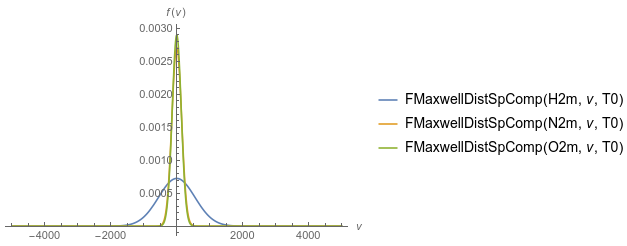
\includegraphics[width=1\linewidth]{1_4_maxw_spcomp_t0.png}}\\
        $T=T_{0}=73K$
    \end{minipage}
    \hfill
    \begin{minipage}[h]{0.47\linewidth}
        \center{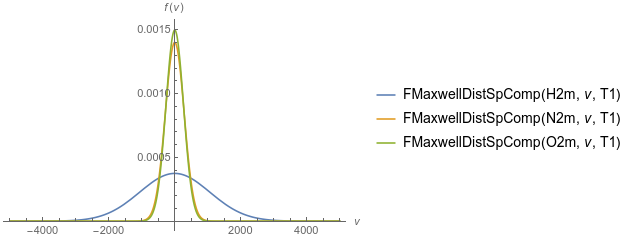
\includegraphics[width=1\linewidth]{1_5_maxw_spcomp_t1.png}}\\
        $T=T_{1}=273K$
    \end{minipage}
    \vfill
    \vspace{6pt}
    \centering 
    \begin{minipage}[h]{0.47\linewidth}
        \center{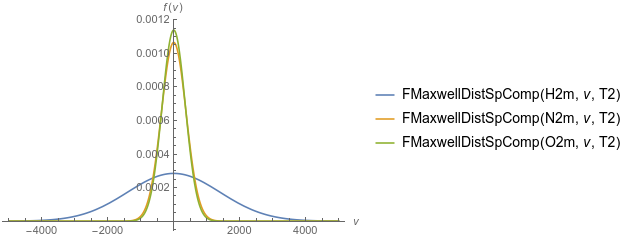
\includegraphics[width=1\linewidth]{1_6_maxw_spcomp_t2.png}}\\
        $T=T_{2}=473K$
    \end{minipage}
\end{figure}

% Часть C

\textit{\textbf{(c) Оценка нормировки распределения Максвелла}}  

Имеем распределения Максвелла по модулю скорости и по проекции скорости из пунктов (a), (b). Тогда, если они нормированы, получим:
\begin{equation*}
    \begin{aligned}
        &\int_{0}^{+\infty} f(v)dv=1, f(v) \text{ --- распределение по модулю скорости}\\
        &\int_{-\infty}^{+\infty} f(v_{i})dv=1, f(v_{i}) \text{ --- распределение по проекции скорости}
    \end{aligned}
\end{equation*}


Листинг программы Matematica:
\begin{center}
    \begin{tabular}{c}
    \begin{lstlisting}
(* Checking the normalization of the distribution functions *)
Integrate[FMaxwellDistAbs[N2m, v, T0], {v, 0, +Infinity}]
Integrate[FMaxwellDistSpComp[N2m, v, T0], {v, -Infinity, +Infinity}]
    \end{lstlisting}
    \end{tabular}
\end{center}

Полученный результат:
\hspace{0pt}
\begin{figure}[H]
    \centering
    \begin{minipage}[h]{0.15\linewidth}
        \center{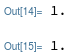
\includegraphics[width=1\linewidth]{1_9_normalisation.png}}\\
    \end{minipage}
\end{figure}

Вывод: распределения нормализованы

% Часть D

\newpage
\textit{\textbf{(d) Определение процента молекул, имеющих модуль скорости из промежутка $[0, v_{\text{ср.кв.}}]$}}

Среднеквадратическая скорость равна:
\begin{equation*}
    v_{\text{ср.кв.}}=\sqrt{\int_{0}^{+\infty} v^{2}f(v)dv} = \sqrt{\frac{3kT}{m}}
\end{equation*}

Зная функцию распределения, получим искомый процент молекул:
\begin{equation*}
    \begin{aligned}
        100\% \cdot &\int_{0}^{v_{\text{ср.кв.}}} f(v)dv, f(v) \text{ --- распределение по модулю скорости}\\
    \end{aligned}
\end{equation*}

Листинг программы Matematica:
\begin{center}
    \begin{tabular}{c}
    \begin{lstlisting}
(*Calculating percentage of molecules with speed in [0, v_avg_sqr]*)
vMS[m_, T_] = Sqrt[3*k*T/m]; (*The mean square speed*)
H2T0SqrSpd = vMS[H2m, T0]; (*The mean square speed for H2 when T=T0*)
Integrate[FMaxwellDistAbs[H2m, v, T0], {v, 0, H2T0SqrSpd}] * 100
    \end{lstlisting}
    \end{tabular}
\end{center}

Полученный результат (60.8\%):
\hspace{0pt}
\begin{figure}[H]
    \centering
    \begin{minipage}[h]{0.2\linewidth}
        \center{
\includegraphics[width=1\linewidth]{1_10_sp0_spSqrAvg.png}}\\
    \end{minipage}
\end{figure}

% Часть E

\textit{\textbf{(e) Определение наиболее вероятной скорости}}

Наиболее вероятная скорость соответствует максимальному значению плотности вероятности распределения.
Тогда решив $\frac{\partial f(v_{\text{н.в.}}) }{\partial v_{\text{н.в.}}} = 0$ относительно $v_{\text{н.в.}}$, получим:
\begin{equation*}
    v_{\text{н.в.}} = \sqrt{\frac{2kT}{m}}
\end{equation*}
Зная функцию распределения, получим искомый процент молекул:
\begin{equation*}
    \begin{aligned}
        100\% \cdot &\int_{0}^{v_{\text{ср.кв.}}} f(v)dv, f(v) \text{ --- распределение по модулю скорости}\\
    \end{aligned}
\end{equation*}

Листинг программы Matematica:
\begin{center}
    \begin{tabular}{c}
    \begin{lstlisting}
(* The most probable speed *)
vP[m_, T_] = Sqrt[2*k*T / m];

(*For different temperatures, H2 gas*)
H2T0MPSpeed = vP[H2m, T0]
H2T1MPSpeed = vP[H2m, T1]
H2T2MPSpeed = vP[H2m, T2]
    \end{lstlisting}
    \end{tabular}
\end{center}

Полученный результат, м/с:
\hspace{0pt}
\begin{figure}[H]
    \centering
    \begin{minipage}[h]{0.2\linewidth}
        \center{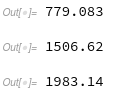
\includegraphics[width=1\linewidth]{1_7_prob_speed.png}}\\
    \end{minipage}
\end{figure}

% Часть F


\textit{\textbf{(f) Вычисление процента молекул со скоростями, отличающимися от наиболее вероятной на 1\%, 5\%}}  

Используя значения наиболее вероятной скорости из пункта (e), получим искомый процент молекул (отличие принято за m процентов):
\begin{equation*}
    \begin{aligned}
        100\% \cdot 
        &\int_{ v_{\text{н.в.}} - v_{\text{н.в.}} \cdot m\% }^{
        v_{\text{н.в.}} + v_{\text{н.в.}} \cdot m\% } f(v)dv, 
        f(v) \text{ --- распределение по модулю скорости}\\
    \end{aligned}
\end{equation*}


Листинг программы Matematica:
\begin{center}
    \begin{tabular}{c}
    \begin{lstlisting}
(* Calculating percintage of moleculas with speeds v_most_prob + - v_most_prob * 1% *)
Integrate[
    FMaxwellDistAbs[H2m, v, T0], 
    {v, H2T0MPSpeed - H2T0MPSpeed * 0.01, 
     H2T0MPSpeed + H2T0MPSpeed * 0.01}] * 100

 (* Calculating percintage of moleculas with speeds v_most_prob + - v_most_prob * 5% *)
Integrate[
    FMaxwellDistAbs[H2m, v, T0], 
    {v, H2T0MPSpeed - H2T0MPSpeed * 0.05, 
     H2T0MPSpeed + H2T0MPSpeed * 0.05}] * 100
    \end{lstlisting}
    \end{tabular}
\end{center}

Полученный результат (1.66\%, 4.97\%):
\hspace{0pt}
\begin{figure}[H]
    \centering
    \begin{minipage}[h]{1\linewidth}
        \center{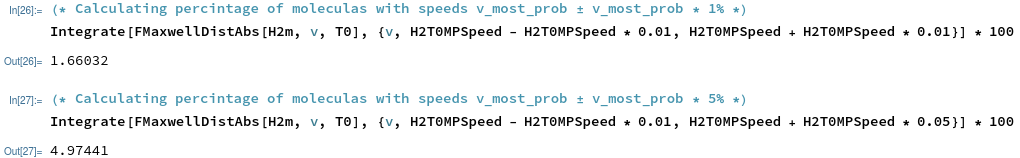
\includegraphics[width=1\linewidth]{1_11_speed_percintage.png}}\\
    \end{minipage}
\end{figure}
